\section{Numerical Experiments} \label{sec:res}

\subsection{Vortex Merging} \label{sec:res.1}
Consider the 2-dimensional incompressible Euler equation \eqref{eq:3.8} on a square domain $\Omega = [0,2\pi]^2$, with periodic boundary conditions. Spatial derivatives are discretized using a Fourier spectral method. To capture the fine details characterizing the solution, $256\times 256$ modes is used. We consider the evolution of three vortices, with the initial structure given by
\begin{equation}\label{eqn:initial_cond_vort}
\omega = \omega_0 + \sum_{i=1}^{3} \alpha_i e^{-\dfrac{\left(x-x_i\right)^{2}+\left(y-y_i\right)^{2}}{\beta^2}}.
\end{equation}
Here, $\omega = \nabla \times u$ is the vorticity, $(x,y)$ represents the spatial coordinates, $\left( x_i, y_i\right)$ is the center of the $i$th vortex, $\alpha_i$ its maximum amplitude, and $\beta$ controls the effective radius of the vortex. In this example, the center of three vortices are 
\begin{equation}
\left( x_1, y_1 \right) = \left(0.75\pi,\pi\right) , \left( x_2, y_2 \right) = \left(1.25\pi,\pi\right), \left( x_3, y_3 \right) = \left(1.25\pi,1.5\pi\right),
\end{equation}
close to the center of the domain. Two of the vortices have a positive spin with $\alpha_1 = \alpha_2 = \pi$ and the third rotates in the opposite direction with $\alpha_3 = -0.5\pi$. The effective radius of all the vortices is set to $\beta = 1 / \pi$. This arrangement of vortices is an interesting initial condition to study the process of vortex merging. This phenomenon is often a result of fast-moving dipoles of vortices with the same spin facing another vortex \cite{filaments_vort2} of opposite spin. The merging process transfers the vorticity from the initial configuration into long, narrow, and spiral-shaped strips of intense vorticity \cite{filaments_vort}. The formation of such thin vorticity filaments in the fluid may pose numerical challenges, due to aliasing. 

In the context of MOR, conservation of energy and stability is crucial to capturing fine structures. With the absence of natural dissipation, straight forward application of MOR techniques for the Euler equation is often unstable.

To define the initial conditions in terms of the velocity components $u$ and the pressure $p$, we define a stream-function $\Psi$, the solution to the equation 
\begin{equation} \label{eq:5.1}
	- \Delta \Psi = \omega.
\end{equation}
The initial velocity is then given by $\nabla \times \Psi$. To solve the stream-function problem \eqref{eq:5.1}, we require $\int_{\Omega} \omega \ dx= 0$. It is easily verified that this requirement implies $\omega_0 = 0.038$. The pressure is recovered by solving the related Poisson pressure equation 
\begin{equation*}
\Delta p = - \nabla \cdot S_{u}(u),
\end{equation*}
obtained by applying the divergence operator to \eqref{eq:3.8} and using the incompressibility condition.
 The implicit midpoint scheme, to mimic the time integration scheme presented in \eqref{eq:3.27}, is used to integrate in time. The merging phenomenon is simulated for a total of $18$ time units using a temporal step $\Delta t=0.004$.

\Cref{compare_different_models} illustrates the evolution of the kinetic energy for the advective, divergence, and the skew-symmetric form of the high-fidelity system. It is observed that only the skew-symmetric form preserves the kinetic energy, confirming the discussion in \Cref{sec:skew.2}.

%%%%%%%%%%%%%%%%%%%%%%%%%%%%%%%%%%%%%%%%%
%%%%% Comparison Skew symmetric, divergence and advective form %%%%%
%%%%%%%%%%%%%%%%%%%%%%%%%%%%%%%%%%%%%%%%%
\begin{figure}[t]
  \centering
  \begin{subfigure}[]{0.47\linewidth}
            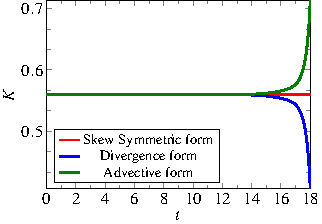
\includegraphics[scale=1]{Figures/paper-figure0.pdf}
%  \begin{tikzpicture}[scale=0.58]
%    \begin{axis}[ylabel=$K$,
%                 xlabel=$t$,
%                 label style={font=\Large},
%                 legend pos=south west,
%                 legend entries={Skew Symmetric form, Divergence form, Advective form},
%                 legend style={font=\large},
%                 width=1.4\linewidth, 
%                 height=1\linewidth,
%                 minor x tick num=1,
%                 minor y tick num=2,	
%                 yticklabel style={/pgf/number format/.cd,fixed,precision=4},
%                 scaled x ticks = true,
%                 enlargelimits=false,
%                 scale only axis]
%                 \addplot[color=red,style=solid,style=ultra thick]  table[x = time, y = energy] {./data/Incompressible_Euler/Energy_compare_formulations/energy_skew_symmetric.txt};
%                 \addplot[color=blue,style=solid,style=ultra thick]  table[x = time, y = energy] {./data/Incompressible_Euler/Energy_compare_formulations/energy_divergence.txt};
%                 \addplot[color=black!50!green,style=solid,style=ultra thick]  table[x = time, y = energy] {./data/Incompressible_Euler/Energy_compare_formulations/energy_convective.txt};
%    \end{axis}%  
%  \end{tikzpicture}
\caption{}
\label{compare_different_models}
\end{subfigure}
  \begin{subfigure}[]{0.47\linewidth}
            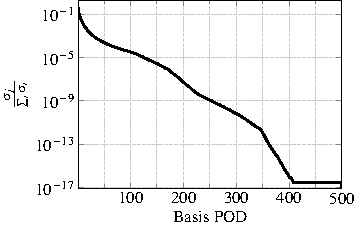
\includegraphics[scale=1]{Figures/paper-figure1.pdf}
%\begin{tikzpicture}[scale=0.58]
%    \begin{semilogyaxis}[ylabel = $\frac{\sigma_j}{\sum_i \sigma_i}$,
%                 xlabel=Basis POD,
%                 label style={font=\Large},
%                 %legend pos=north east,
%                 %legend entries={$k=24$ Div,$k=102$ Div,$k=201$ Div,$k=24$ Skew,$k=102$ Skew,$k=201$ Skew},
%                 legend style={font=\large},
%                 grid=both,
%                 ticks=both,
%                 width=1.4\linewidth, 
%                 height=1\linewidth,
%                 minor x tick num=1,
%                 minor y tick num=2,	
%                 yticklabel style={/pgf/number format/.cd,fixed,precision=9},
%                 scaled x ticks = true,
%                 enlargelimits=false,
%                 scale only axis,
%                 ymin=0,
%                 ymax = 2,
%                 samples = 100]
%                 \addplot[color=black,style=solid,style=ultra thick]  table[x = x, y = s] {./data/Incompressible_Euler/Singular_values/sv.txt};
%    \end{semilogyaxis}
%\end{tikzpicture}
\caption{}
\label{singular_values_decay}
\end{subfigure}
  \caption{(\protect\subref{compare_different_models}) The kinetic energy $K$ for the advective, divergence and the skew-symmetric formulations. (\protect\subref{singular_values_decay}) The decay of the singular values for the vortex merging. }
  \label{fig:unstable_full_models}
\end{figure}
A total of $5000$ temporal snapshots is used to construct a reduced basis, following the process discussed in \Cref{sec:mor}. The decay of the singular values, used as an indication of the reducibility of the problem, is presented in \Cref{singular_values_decay}. The first $35$ POD modes corresponds to over $99\%$ of the modes of the high fidelity solution. This suggests that an accurate reduced system can be constructed using a small number of basis vectors. To illustrate the effectiveness of the method, smaller bases are also considered.

For a qualitative analysis, in Figure \ref{fig:snap_solution_incompressible_Euler}, four solutions at different times are shown for the high fidelity system and the reduced system with $k=17$ and $k=35$ modes. The overall dynamics of the problem, and in particular the formation and development of vorticity filaments, are correctly represented, even with a moderate number of basis vectors. Although small details are not captured by the reduced system with a small number of basis vectors, the position and the spreading of the vortices are comparable. 

%%%%%%%%%%%%%%%%%%%%%%%%%%%%%%%%%%%%%%%%%%%%
%%%%%%%%%%%%%% Snapshots of merging process %%%%%%%%%%%%%%
%%%%%%%%%%%%%%%%%%%%%%%%%%%%%%%%%%%%%%%%%%%%
\begin{figure}[t]
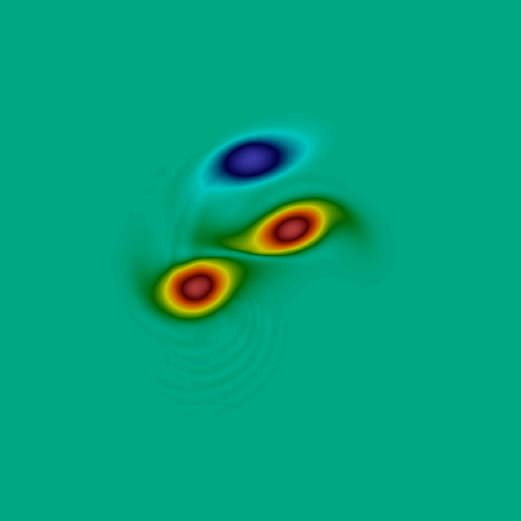
\includegraphics[scale=0.06]{data/Incompressible_Euler/Snapshots/red_17_2.png}\hspace{1em}
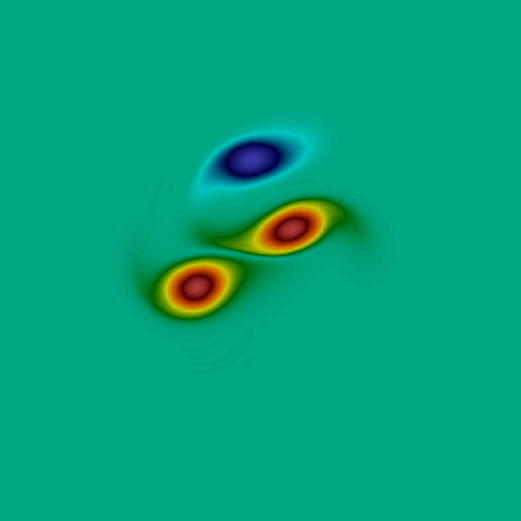
\includegraphics[scale=0.06]{data/Incompressible_Euler/Snapshots/red_35_2.png}\hspace{1em}
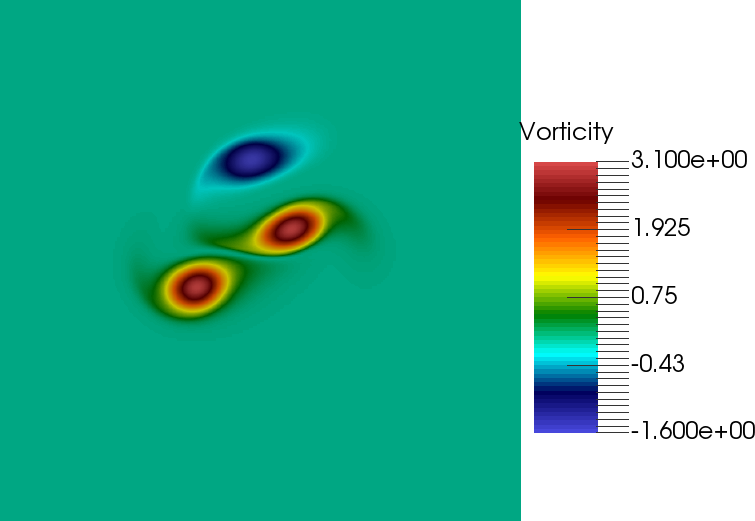
\includegraphics[scale=0.06]{data/Incompressible_Euler/Snapshots/Full_2.png}\\

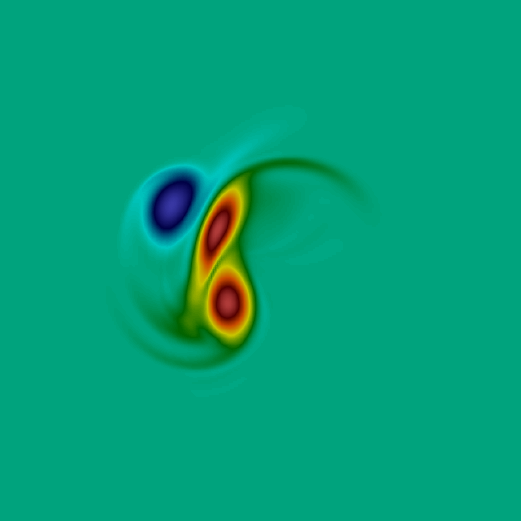
\includegraphics[scale=0.06]{data/Incompressible_Euler/Snapshots/red_17_3.png}\hspace{1em}
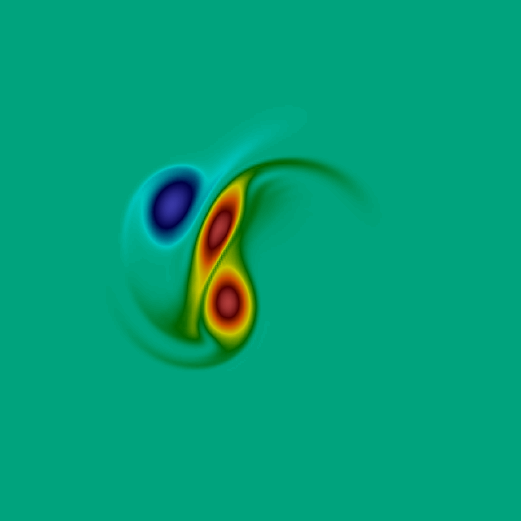
\includegraphics[scale=0.06]{data/Incompressible_Euler/Snapshots/red_35_3.png}\hspace{1em}
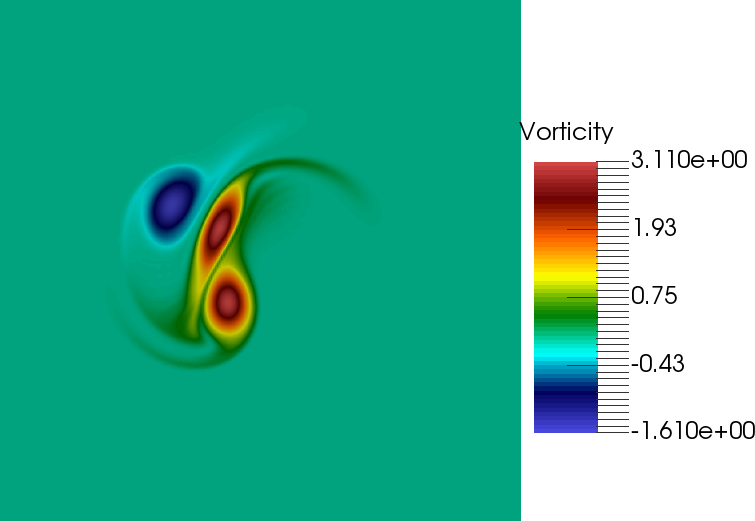
\includegraphics[scale=0.06]{data/Incompressible_Euler/Snapshots/Full_3.png}\\

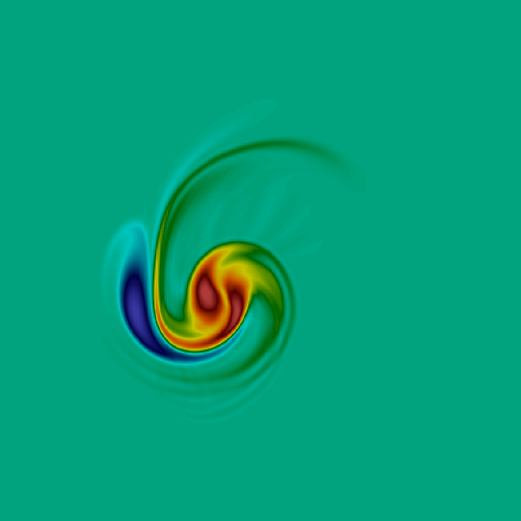
\includegraphics[scale=0.06]{data/Incompressible_Euler/Snapshots/red_17_4.png}\hspace{1em}
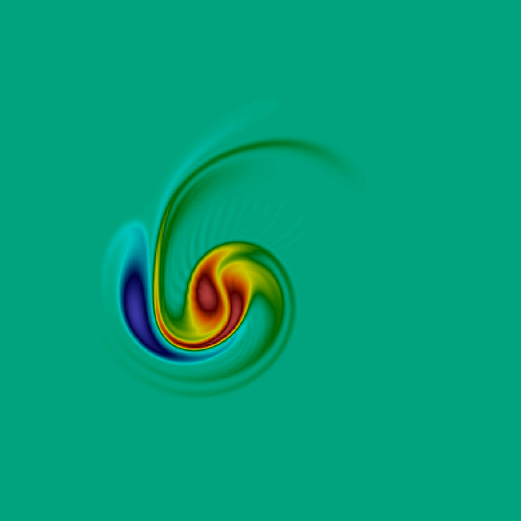
\includegraphics[scale=0.06]{data/Incompressible_Euler/Snapshots/red_35_4.png}\hspace{1em}
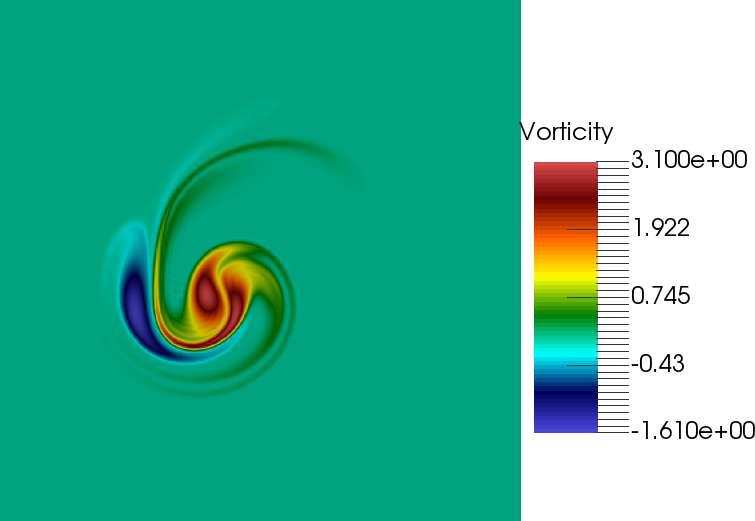
\includegraphics[scale=0.06]{data/Incompressible_Euler/Snapshots/Full_4.png}\\

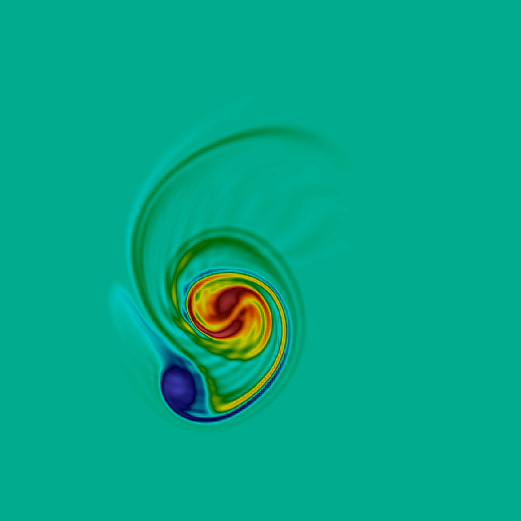
\includegraphics[scale=0.06]{data/Incompressible_Euler/Snapshots/red_17_5.png}\hspace{1em}
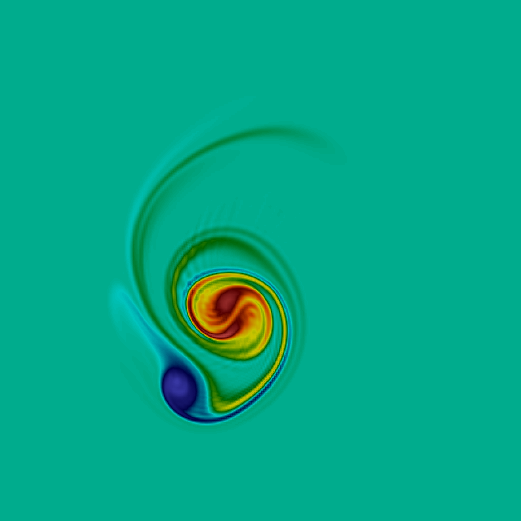
\includegraphics[scale=0.06]{data/Incompressible_Euler/Snapshots/red_35_5.png}\hspace{1em}
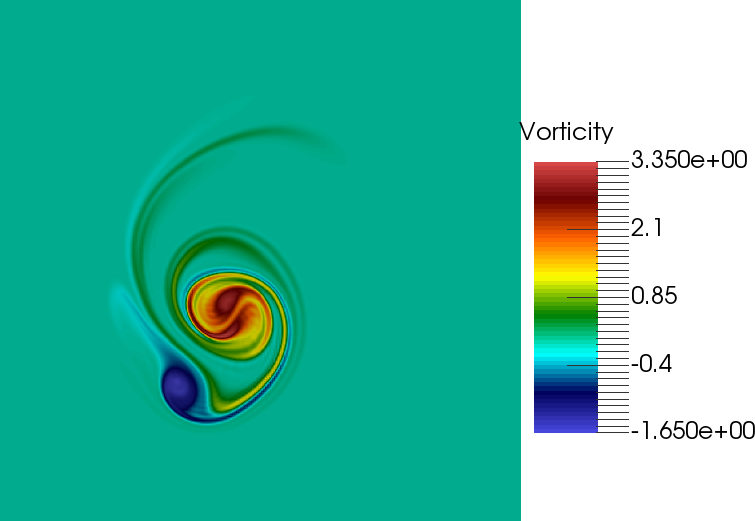
\includegraphics[scale=0.06]{data/Incompressible_Euler/Snapshots/Full_5.png}

\caption{Snapshots of the high-fidelity system and the reduced system at $t=\left\{ 4,8,12,18 \right\}$. From left to right: the solution of the reduced model with $k=17$, $k=35$ and the high fidelity solution.}
\label{fig:snap_solution_incompressible_Euler}
\end{figure}


%%%%%%%%%%%%%%%%%%%%%%%%%%%%%%%%%%%%%%%%%%
%%%%%%%%%% Singular values decay merging vorteces %%%%%%%%%%%
%%%%%%%%%%%%%%%%%%%%%%%%%%%%%%%%%%%%%%%%%%
\Cref{fig:approx_error_incompressible_Euler} shows the $L^2$ error between the high-fidelity solution and the reduced solution. The error decreases, consistently, as the number of basis vectors increases. Furthermore, the accuracy is maintained over the period of time integration.

The conservation of the kinetic energy is presented in \Cref{fig:energy_error_incompressible_Euler}. Even for a small number of basis vectors, where the solution is not well approximated, the kinetic energy remains constant. Furthermore, the error in the kinetic energy, due to MOR, is constant in time. This is central for the robustness of the reduced system during long time-integration.


%%%%%%%%%%%%%%%%%%%%%%%%%%%%%%%%%%%%%%%%%%%
%%%%%%%%%% Approximation error and energy conservation %%%%%%%%%%
%%%%%%%%%%%%%%%%%%%%%%%%%%%%%%%%%%%%%%%%%%%
\begin{figure}[t]
\centering
\begin{subfigure}[]{0.47\linewidth}
          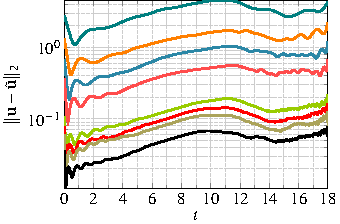
\includegraphics[scale=1]{Figures/paper-figure2.pdf}
%\begin{tikzpicture}[scale=0.58]
%    \begin{semilogyaxis}[ylabel = $\| \mathbf{u}-\tilde{\mathbf{u}}\|_2$,
%                 xlabel=$t$,
%                 label style={font=\Large},
%                 legend style={font=\large},
%                 grid=both,
%                 ticks=both,
%                 width=1.4\linewidth, 
%                 height=1.0\linewidth,
%                 minor x tick num=1,
%                 minor y tick num=2,	
%                 yticklabel style={/pgf/number format/.cd,fixed,precision=9},
%                 scaled x ticks = true,
%                 enlargelimits=false,
%                 scale only axis,
%                 samples = 100,
%                 cycle list name=exotic]
%                 \addplot+[style=solid,style=ultra thick]  table[x = time, y = error] {./data/Incompressible_Euler/Approximation_Error/err_5.txt};
%                 \addplot+[style=solid,style=ultra thick]  table[x = time, y = error] {./data/Incompressible_Euler/Approximation_Error/err_8.txt};
%                 \addplot+[style=solid,style=ultra thick]  table[x = time, y = error] {./data/Incompressible_Euler/Approximation_Error/err_11.txt};
%                 \addplot+[style=solid,style=ultra thick]  table[x = time, y = error] {./data/Incompressible_Euler/Approximation_Error/err_14.txt};
%                 \addplot+[style=solid,style=ultra thick]  table[x = time, y = error] {./data/Incompressible_Euler/Approximation_Error/err_23.txt};
%                 \addplot+[style=solid,style=ultra thick]  table[x = time, y = error] {./data/Incompressible_Euler/Approximation_Error/err_26.txt};
%                 \addplot+[style=solid,style=ultra thick]  table[x = time, y = error] {./data/Incompressible_Euler/Approximation_Error/err_29.txt};
%                 \addplot+[style=solid,style=ultra thick]  table[x = time, y = error] {./data/Incompressible_Euler/Approximation_Error/err_35.txt};
%    \end{semilogyaxis}
%\end{tikzpicture}
\caption{}
\label{fig:approx_error_incompressible_Euler}
\end{subfigure} \hfill
\begin{subfigure}[]{0.47\linewidth}
          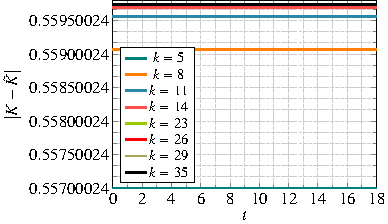
\includegraphics[scale=1]{Figures/paper-figure3.pdf}
%\begin{tikzpicture}[scale=0.58]
%    \begin{axis}[ylabel = $|K-\tilde{K}|$,
%                 xlabel=$t$,
%                 label style={font=\Large},
%                 legend pos=south west,
%                 legend entries={$k=5$ , $k=8$, $k=11$, $k=14$, $k=23$, $k=26$, $k=29$, $k=35$},
%                 legend style={font=\large},
%                 grid=both,
%                 ticks=both,
%                 width=1.4\linewidth, 
%                 height=1.0\linewidth,
%                 minor x tick num=1,
%                 minor y tick num=2,	
%                 yticklabel style={/pgf/number format/.cd,fixed,precision=9},
%                 scaled x ticks = true,
%                 enlargelimits=false,
%                 scale only axis,
%                 ymax = 0.5598,
%                 samples = 100,
%                 cycle list name=exotic]
%                 \addplot+[style=solid,style=ultra thick]  table[x = time, y = error] {./data/Incompressible_Euler/Energy_conservation/ene_full_5.txt};
%                 \addplot+[style=solid,style=ultra thick]  table[x = time, y = error] {./data/Incompressible_Euler/Energy_conservation/ene_full_8.txt};
%                 \addplot+[style=solid,style=ultra thick]  table[x = time, y = error] {./data/Incompressible_Euler/Energy_conservation/ene_full_11.txt};
%                 \addplot+[style=solid,style=ultra thick]  table[x = time, y = error] {./data/Incompressible_Euler/Energy_conservation/ene_full_14.txt};
%                 \addplot+[style=solid,style=ultra thick]  table[x = time, y = error] {./data/Incompressible_Euler/Energy_conservation/ene_full_23.txt};
%                 \addplot+[style=solid,style=ultra thick]  table[x = time, y = error] {./data/Incompressible_Euler/Energy_conservation/ene_full_26.txt};
%                 \addplot+[style=solid,style=ultra thick]  table[x = time, y = error] {./data/Incompressible_Euler/Energy_conservation/ene_full_29.txt};
%                 \addplot+[style=solid,style=ultra thick]  table[x = time, y = error] {./data/Incompressible_Euler/Energy_conservation/ene_full_35.txt};
%    \end{axis}
%\end{tikzpicture}
\caption{}
\label{fig:energy_error_incompressible_Euler}
\end{subfigure}
\label{fig:energy_approx_err}
\caption{(\protect\subref{fig:approx_error_incompressible_Euler}) Evolution of $L_2$ error in velocity, between the high-fidelity system and the reduced system. (\protect\subref{fig:energy_error_incompressible_Euler}) Conservation of the kinetic energy.}
\end{figure}


\subsection{2D Kelvin-Helmholtz instability}
Consider the 2-dimensional compressible Euler equation \eqref{eq:3.18} in a periodic square box $[0,1]^2$. Unlike the incompressible example in \Cref{sec:res.1}, a centered finite difference scheme of fourth order is used to discretize \eqref{eq:3.18}. The physical domain is discretized into a grid of $256\times 256$ nodes.

The initial velocity field is given by
\begin{equation*}
\begin{cases}
& \mathbf{r} = 
\begin{cases}
& 2, \text{ if } 0.25<y<0.75,\\
& 1, \text{ otherwise },
\end{cases}
\\
& \mathbf{u}_x = a \sin(4\pi y) \left( e^{-\dfrac{(y-0.25)^2}{2\sigma^2}} + e^{-\dfrac{(y-0.75)^2}{2\sigma^2}} \right),\\
& \mathbf{u}_y = 
\begin{cases}
& 0.5, \text{ if } 0.25<y<0.75,\\
& -0.5, \text{ otherwise },
\end{cases},
\\
& \mathbf{p} = 2.5,\\
\end{cases}
\end{equation*}
where $a=0.1$ and $\sigma=5\sqrt{2}\cdot 10^{-3}$. This corresponds to contacting streams of fluid with different densities. For specific choices of parameters describing the jets, fine structures and vortices emerges at the interface between the streams. Such an instability is referred to as the Kelvin-Helmholtz instability \cite{HHS}.

As centered schemes are often dissipation free, resolving the discontinuous initial data requires some artificial viscosity. In the high-fidelity model, the method discussed in \cite{artificial_dissipation}\edit{, based on a derivative-based model,} is used as an artificial viscosity. However, at the level of the reduced system, this is replaced with a low pass filter on the expansion coefficients of POD basis vectors. \edit{The last $5\%$ of the POD modes are put to zero every $20$ time iterations. The reason for the different treatment is that we want to avoid the reconstruction of the derivative of the solution in the full space during the integration of the reduced system.}

The fully discrete skew-symmetric form \eqref{eq:3.27} is used as a time marching scheme with $\Delta t = 5 \cdot 10^{-4}$ over a period of $1$ time unit.
\edit{A total of $500$ snapshots have been used for the computation of the basis in the offline stage.}

\Cref{fig:error_decay_KH} illustrates that the accuracy of the method consistently improves as a higher number of POD basis modes are considered. Furthermore, the skew-symmetric form preserves the accuracy over the period of time integration. It is observed in \Cref{fig:snap_solution_KH} that all features of the flow are correctly represented in the reduced system, even with a low number of basis vectors.

\begin{figure}[t]
\centering
\begin{subfigure}[]{0.48\linewidth}
          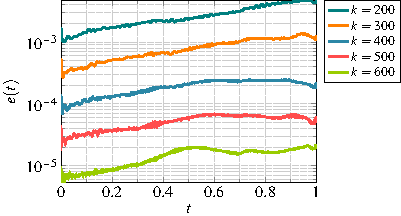
\includegraphics[scale=1]{Figures/paper-figure4.pdf}
%  \begin{tikzpicture}[scale=0.55]
%    \begin{semilogyaxis}[xlabel=$t$,
%                 ylabel=$e(t)$,
%                 label style={font=\Large},
%                 legend pos=outer north east,
%                 legend style={font=\large},
%                 legend entries={$k=200$,$k=300$,$k=400$,$k=500$,$k=600$},
%                 grid=both,
%                 ticks=both,
%                 width=1.4\linewidth, 
%                 height=1.0\linewidth,
%                 minor x tick num=1,
%                 minor y tick num=2,	
%                 yticklabel style={/pgf/number format/.cd,fixed,precision=9},
%                 scaled x ticks = true,
%                 enlargelimits=false,
%                 scale only axis,
%                 cycle list name=exotic]
%                 \addplot+[style=solid,style=ultra thick]  table[x = time, y = quantity] {./data/Compressible_Euler/KH/error/error_200.txt};  
%                 \addplot+[style=solid,style=ultra thick]  table[x = time, y = quantity] {./data/Compressible_Euler/KH/error/error_300.txt};      
%                 \addplot+[style=solid,style=ultra thick]  table[x = time, y = quantity] {./data/Compressible_Euler/KH/error/error_400.txt}; 
%                 \addplot+[style=solid,style=ultra thick]  table[x = time, y = quantity] {./data/Compressible_Euler/KH/error/error_500.txt};      
%                 \addplot+[style=solid,style=ultra thick]  table[x = time, y = quantity] {./data/Compressible_Euler/KH/error/error_600.txt};               
%    \end{semilogyaxis}%  
%  \end{tikzpicture}
\end{subfigure}
\caption{Evolution in time of the error  between the high fidelity solution of the Kelvin-Helmoltz and the reduced solution for different number of basis $k$. As error measure we use $e(t)=\sqrt{\|\mathbf{r}-\mathbf{r}^r\|^2+\|\mathbf{u_xr}-\mathbf{u_xr}^r\|^2 + \|\mathbf{u_yr}-\mathbf{u_yr}^r\|^2 + \|\mathbf{p}-\mathbf{p}^r\|^2}$.}
\label{fig:error_decay_KH}
\end{figure}

Conservation of mass, momentum and energy is presented in \Cref{fig:conservation_DEIM}. The accuracy of the method in approximating these invariants improves as the size of the basis is increased. Furthermore, \Cref{energy_error_KH} shows how the kinetic energy associated with the reduced system mimic the kinetic energy of the high-fidelity system. This helps to ensure the correct evolution of kinetic energy, and thus, the internal energy.
 
\begin{figure}
  \centering
  \begin{subfigure}[]{0.48\linewidth}
            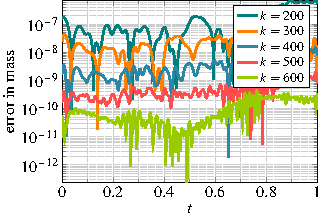
\includegraphics[scale=1]{Figures/paper-figure5.pdf}
%  \begin{tikzpicture}[scale=0.55]
%    \begin{semilogyaxis}[ylabel = error in mass,
%                 xlabel=$t$,
%                 label style={font=\Large},
%                 legend pos=north east,
%                 legend entries={$k=200$ ,$k=300$, $k=400$,$k=500$,$k=600$},
%                 legend style={font=\large},
%                 grid=both,
%                 ticks=both,
%                 width=1.4\linewidth, 
%                 height=1.0\linewidth,
%                 minor x tick num=1,
%                 minor y tick num=2,	
%                 %yticklabel style={/pgf/number format/.cd,fixed,precision=9},
%                 scaled x ticks = true,
%                 enlargelimits=false,
%                 scale only axis,
%                 cycle list name=exotic]
%                 \addplot+[style=solid,style=ultra thick]  table[x = time, y = quantity] {./data/Compressible_Euler/KH/conserved_quantities/mass_red_200.txt};
%                 \addplot+[style=solid,style=ultra thick]  table[x = time, y = quantity] {./data/Compressible_Euler/KH/conserved_quantities/mass_red_300.txt};
%                 \addplot+[style=solid,style=ultra thick]  table[x = time, y = quantity] {./data/Compressible_Euler/KH/conserved_quantities/mass_red_400.txt};
%                 \addplot+[style=solid,style=ultra thick]  table[x = time, y = quantity] {./data/Compressible_Euler/KH/conserved_quantities/mass_red_500.txt};
%                 \addplot+[style=solid,style=ultra thick]  table[x = time, y = quantity] {./data/Compressible_Euler/KH/conserved_quantities/mass_red_600.txt};
%    \end{semilogyaxis}%  
%  \end{tikzpicture}
  \caption{}
  \label{mass_error_KH}
  \end{subfigure}\hfill
  \begin{subfigure}[]{0.48\linewidth}
            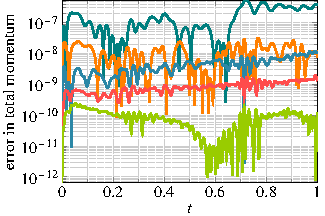
\includegraphics[scale=1]{Figures/paper-figure6.pdf}
%  \begin{tikzpicture}[scale=0.55]
%    \begin{semilogyaxis}[ylabel = error in total momentum,
%                 xlabel=$t$,
%                 label style={font=\Large},
%                 legend pos=north east,
%%                 legend entries={$k=200$ Conv,$k=201$ Conv},
%                 legend style={font=\large},
%                 grid=both,
%                 ticks=both,
%                 width=1.4\linewidth, 
%                 height=1.0\linewidth,
%                 minor x tick num=1,
%                 minor y tick num=2,	
%                 %yticklabel style={/pgf/number format/.cd,fixed,precision=9},
%                 scaled x ticks = true,
%                 enlargelimits=false,
%                 scale only axis,
%                 cycle list name=exotic]
%                 \addplot+[style=solid,style=ultra thick]  table[x = time, y = quantity] {./data/Compressible_Euler/KH/conserved_quantities/momentum_red_200.txt};
%                 \addplot+[style=solid,style=ultra thick]  table[x = time, y = quantity] {./data/Compressible_Euler/KH/conserved_quantities/momentum_red_300.txt};
%                 \addplot+[style=solid,style=ultra thick]  table[x = time, y = quantity] {./data/Compressible_Euler/KH/conserved_quantities/momentum_red_400.txt};
%                 \addplot+[style=solid,style=ultra thick]  table[x = time, y = quantity] {./data/Compressible_Euler/KH/conserved_quantities/momentum_red_500.txt};
%                 \addplot+[style=solid,style=ultra thick]  table[x = time, y = quantity] {./data/Compressible_Euler/KH/conserved_quantities/momentum_red_600.txt};
%    \end{semilogyaxis}%  
%  \end{tikzpicture}
  \caption{}
  \label{momentum_error_KH}
  \end{subfigure}
  
  \begin{subfigure}[]{0.48\linewidth}
            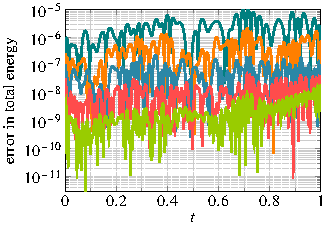
\includegraphics[scale=1]{Figures/paper-figure7.pdf}
%  \begin{tikzpicture}[scale=0.55]
%    \begin{semilogyaxis}[ylabel = error in total energy,
%                 xlabel=$t$,
%                 label style={font=\Large},
%                 legend pos=north east,
%%                 legend entries={$k=200$ Conv,$k=201$ Conv},
%                 legend style={font=\large},
%                 grid=both,
%                 ticks=both,
%                 width=1.4\linewidth, 
%                 height=1.0\linewidth,
%                 minor x tick num=1,
%                 minor y tick num=2,	
%                 %yticklabel style={/pgf/number format/.cd,fixed,precision=9},
%                 scaled x ticks = true,
%                 enlargelimits=false,
%                 scale only axis,
%                 cycle list name=exotic]
%                 \addplot+[style=solid,style=ultra thick]  table[x = time, y = quantity] {./data/Compressible_Euler/KH/conserved_quantities/energy_red_200.txt};
%                 \addplot+[style=solid,style=ultra thick]  table[x = time, y = quantity] {./data/Compressible_Euler/KH/conserved_quantities/energy_red_300.txt};
%                 \addplot+[style=solid,style=ultra thick]  table[x = time, y = quantity] {./data/Compressible_Euler/KH/conserved_quantities/energy_red_400.txt};
%                 \addplot+[style=solid,style=ultra thick]  table[x = time, y = quantity] {./data/Compressible_Euler/KH/conserved_quantities/energy_red_500.txt};
%                 \addplot+[style=solid,style=ultra thick]  table[x = time, y = quantity] {./data/Compressible_Euler/KH/conserved_quantities/energy_red_600.txt};
%    \end{semilogyaxis}%  
%  \end{tikzpicture}
   \caption{}
  \label{energy_error_KH}
  \end{subfigure}
\caption{Difference between the high fidelity solution of the Kelvin-Helmholtz problem and the reduced solution of the mass (\protect\subref{mass_error_KH}), the momentum (\protect\subref{momentum_error_KH}), and the total energy (\protect\subref{energy_error_KH}).}
\label{fig:conservation_DEIM}
\end{figure}

%%%%%%%%%%%%%%%%%%%%%%%%%%%%%%%%%%%%%
%%%%%%%%%%%%%% Snapshots of KH %%%%%%%%%%%%%%
%%%%%%%%%%%%%%%%%%%%%%%%%%%%%%%%%%%%%
\begin{figure}[h!]
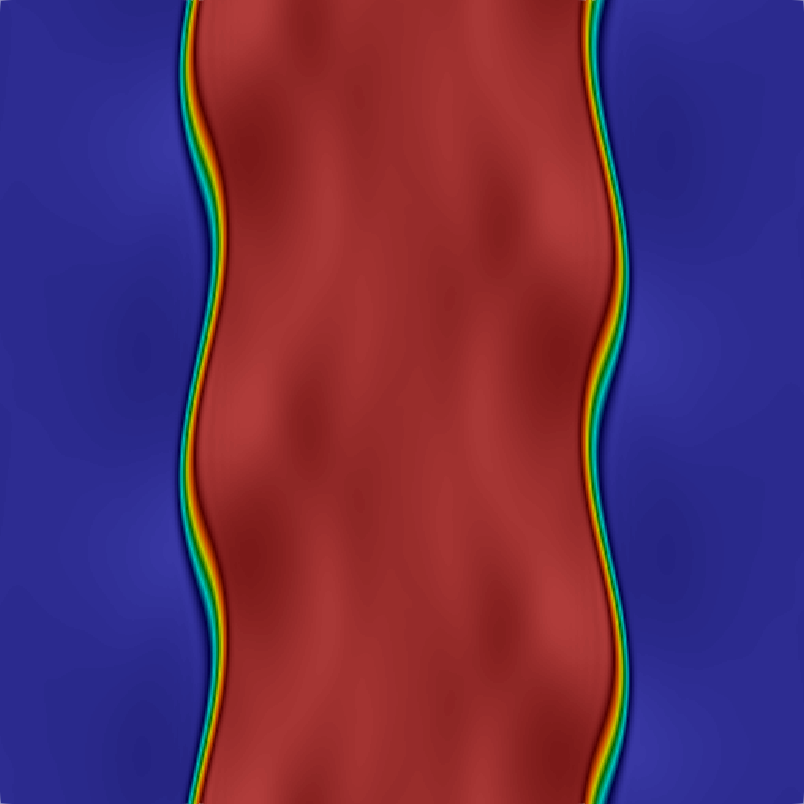
\includegraphics[scale=0.115]{data/Compressible_Euler/KH/Snapshots/density_200_307.png}\hspace{1em}
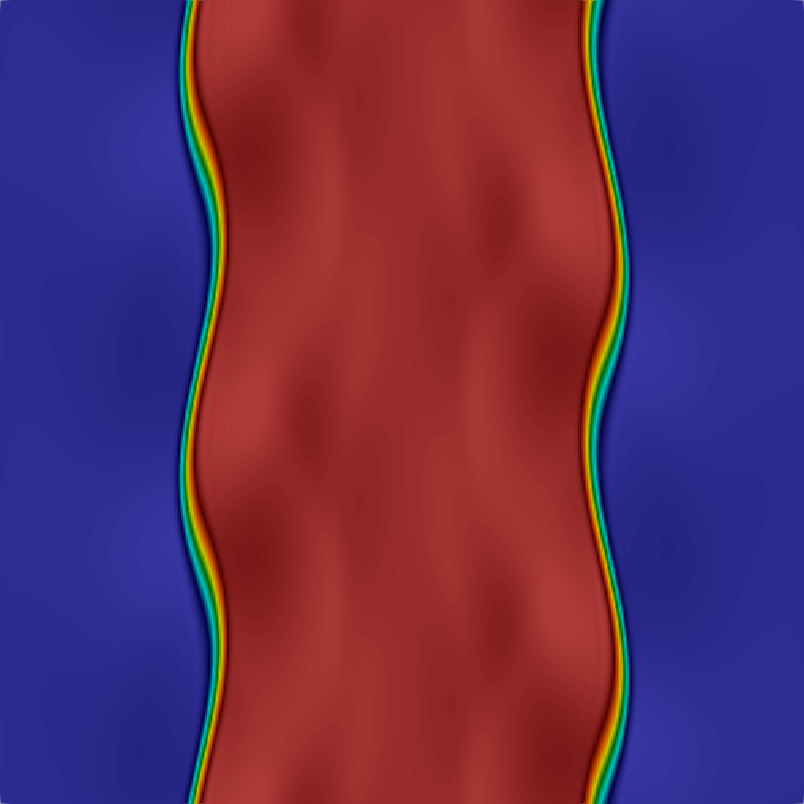
\includegraphics[scale=0.115]{data/Compressible_Euler/KH/Snapshots/density_500_307.png}\hspace{1em}
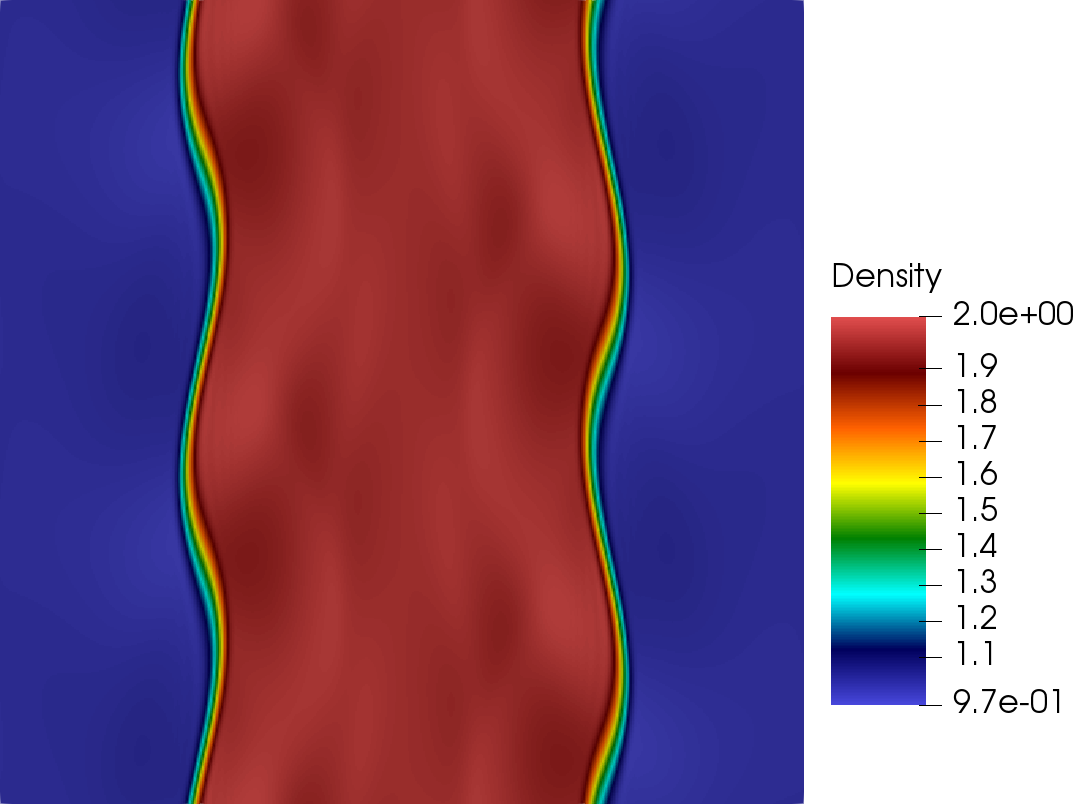
\includegraphics[scale=0.115]{data/Compressible_Euler/KH/Snapshots/density_exact_307.png}\\

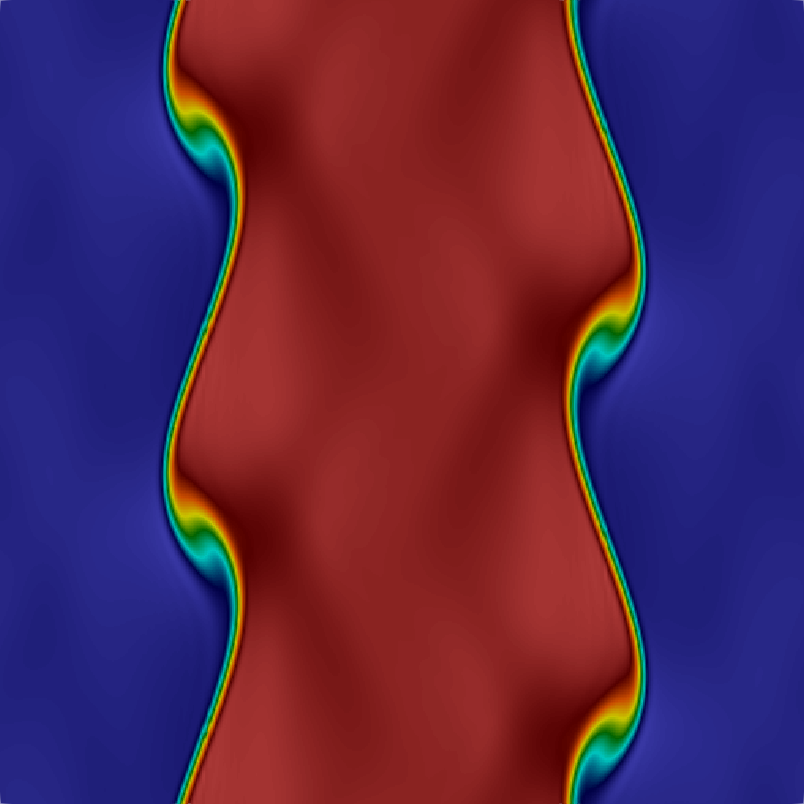
\includegraphics[scale=0.115]{data/Compressible_Euler/KH/Snapshots/density_200_461.png}\hspace{1em}
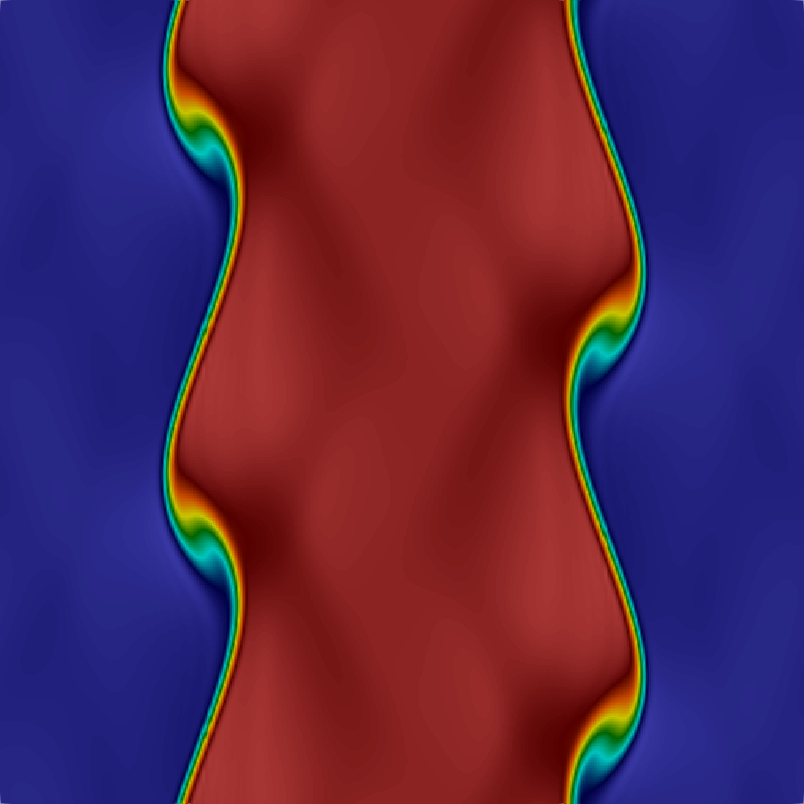
\includegraphics[scale=0.115]{data/Compressible_Euler/KH/Snapshots/density_500_461.png}\hspace{1em}
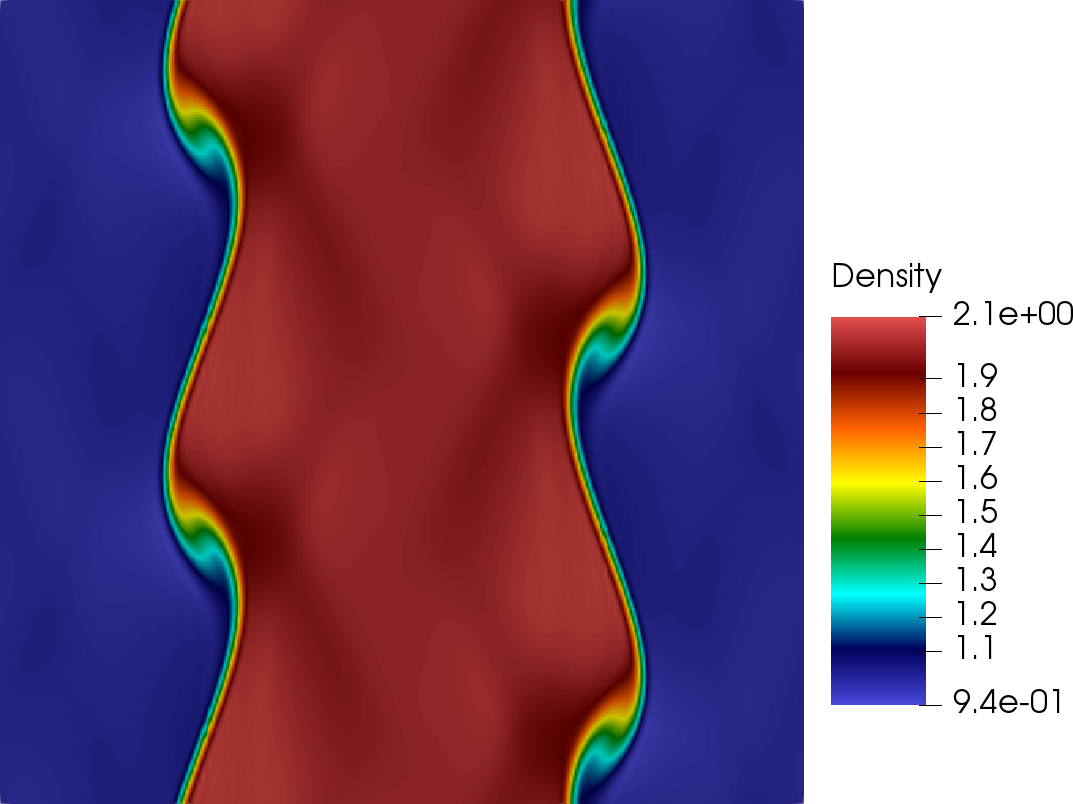
\includegraphics[scale=0.115]{data/Compressible_Euler/KH/Snapshots/density_exact_461.png}\\


\includegraphics[scale=0.115]{data/Compressible_Euler/KH/Snapshots/density_200_614.png}\hspace{1em}

\includegraphics[scale=0.115]{data/Compressible_Euler/KH/Snapshots/density_500_614.png}\hspace{1em}
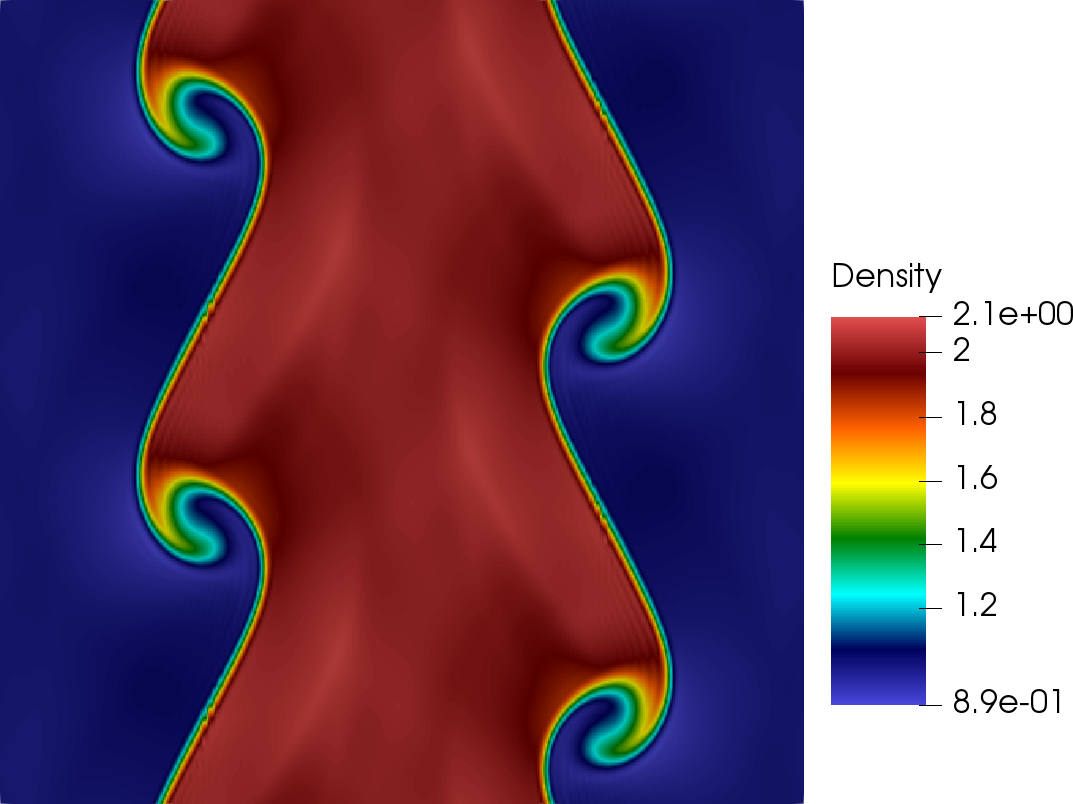
\includegraphics[scale=0.115]{data/Compressible_Euler/KH/Snapshots/density_exact_614.png}\\


\includegraphics[scale=0.115]{data/Compressible_Euler/KH/Snapshots/density_200_768.png}\hspace{1em}

\includegraphics[scale=0.115]{data/Compressible_Euler/KH/Snapshots/density_500_768.png}\hspace{1em}
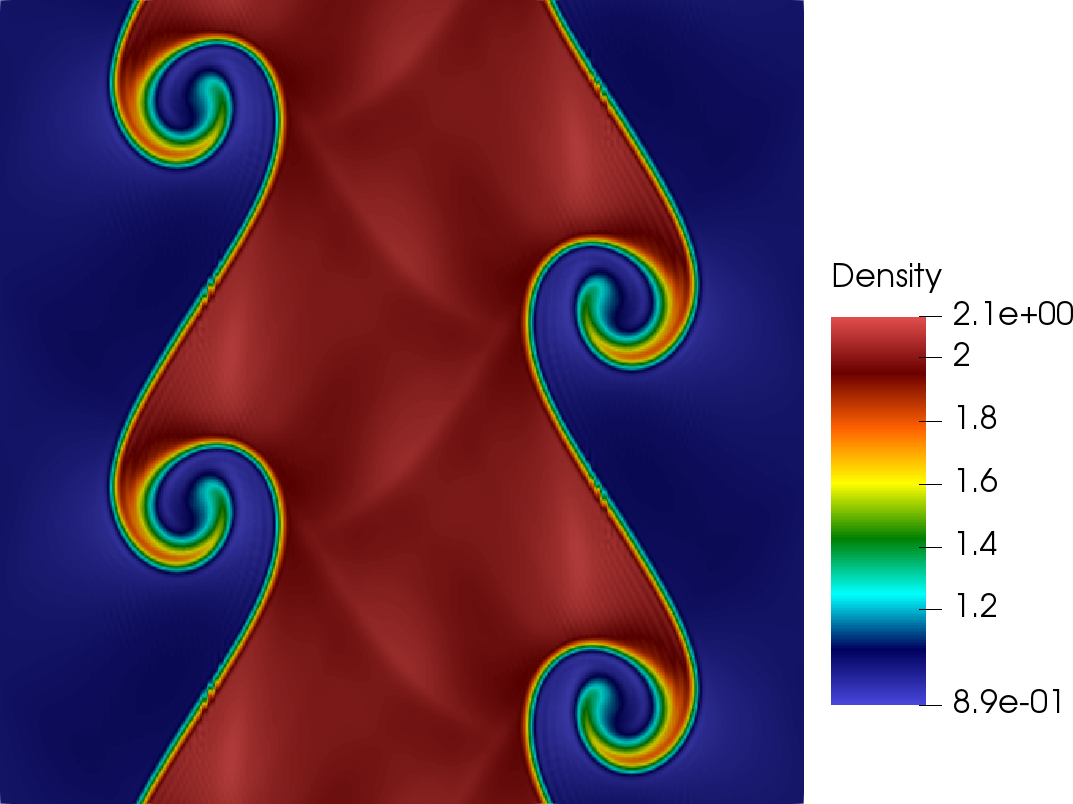
\includegraphics[scale=0.115]{data/Compressible_Euler/KH/Snapshots/density_exact_768.png}

\caption{Solutions of the Kelvin-Helmholtz problem at $t=\left\{ 0.4, 0.6, 0.8, 1 \right\}$. From left to right we show the solution of the reduced model with $k=200$, $k=500$ and the high fidelity solution.}
\label{fig:snap_solution_KH}
\end{figure}


\subsection{1D Shock problem}
In this section we study the 1-dimensional compressible Euler problem, \eqref{eq:3.18} without viscous terms, with a steady state discontinuous solution. This is in preparation for \Cref{sec:5.res.4}, where development and propagation of shock waves is discussed. Here we asses how the skew-symmetric form of \eqref{eq:3.18} can recover moving discontinuities at the level of the reduced system. Consider a periodic boundary conditions on $\Omega = [0,1]$ with the initial condition
\begin{equation*}
\begin{cases}
& \mathbf{r} = 0.5+0.2 \cos(2\pi x),\\
& \mathbf{u} = 1.5,\\
& \mathbf{p} = 0.5+0.2 \sin(2\pi x).\\
\end{cases}
\end{equation*}
The domain is discretized into $N=2000$ nodes and a centered finite differences scheme is used to assemble the discrete Euler equation in skew-symmetric form, as discussed in \Cref{sec:skew.3}. 

The fully discrete skew-symmetric form \eqref{eq:3.27} is used for time integration over a time interval $[0,0.3]$. To resolve the discontinuous solution we use an artificial viscosity with $\tau = \mu \partial u / \partial x$, where $\mu = 0.5 \cdot 10^{-4}$. \edit{Regarding the reduction procedure, $1000$ snapshots of the numerical solution given by the high fidelity method have been collected.}

		\Cref{fig:energy_pres_1D} shows the evolution of conserved quantities for the high-fidelity and reduced system. Here, the high-fidelity model is also considered in the divergence and advective form in addition to the skew-symmetric form. It is clear that when the reduced systems is not in skew-symmetric form, it violates conservation of mass, momentum, and energy. Even while the high-fidelity systems in divergence and advective forms are stable, the constructed reduced system is unstable, independent on the number of basis vectors. On the other hand, the skew-symmetric form yields a stable and conservative reduce system. Note that the loss in the energy associated with the skew-symmetric form, illustrated in \Cref{conservation_1D_focus}, is due to the application of an artificial viscosity. 

\Cref{error_behaviour_1D} shows the total error, when the reduced system captures a discontinuous solution at $t=0.16$. It is observed that the formation of a discontinuity affects the accuracy of the method. This is expected as a sharp gradient is approximated by a relatively few POD modes. However, the method remains robust and stable during the period of time integration.

In \Cref{fig:snaps_1D_Euler} we compare the numerical artifacts of different formulations of the Euler equation. The advective formulation is not presented since it does not yield a stable reduced system. It is observed that the reduced system based on the skew-symmetric formulation accurately represent the overall behavior of the high-fidelity solution. On the other hand, a Gibbs-type error \cite{thompson1992fourier} appears near sharp gradients, for the reduced system based on the divergence form of the Euler equation. The well-representation of the skew-symmetric form is due the low aliasing error property. 

As discussed in \Cref{sec:mor_skew}, the DEIM approximation needed for an efficient evaluation of the nonlinear components of \eqref{eq:3.18}, can affect the conservation properties of the skew-symmetric form. \Cref{fig:singular_values_decay_1D} shows the decay of the singular values of the nonlinear snapshots. The decay of these snapshots is significantly slower than the temporal snapshots of \eqref{eq:3.18}. This indicates that to maintain the accuracy of the reduced system, the DEIM basis should be chosen richer than the POD basis. \Cref{error_DEIM} and \Cref{energy_DEIM} present the error and the conservation of total energy when the DEIM is used to approximate the nonlinear term. The conservation of energy is recovered once DEIM approximates the nonlinear terms with enough accuracy. 
In this numerical experiment, evaluation of the nonlinear terms in \eqref{eq:3.18} using the DEIM is ten times faster than the high-fidelity evaluation.

%%%%%%%%%%%%%%%%%%%%%%%%%%%%%%%%%%%%%%%%%%%%
%%%%%%%%%%%%% Mass, Total momentum & Energy %%%%%%%%%%%%%%
%%%%%%%%%%%%%%%%%%%%%%%%%%%%%%%%%%%%%%%%%%%%
\begin{figure}
  \centering
  % MASS
  \begin{subfigure}[]{0.48\linewidth}
            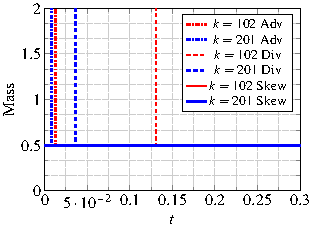
\includegraphics[scale=1]{Figures/paper-figure8.pdf}
%  \begin{tikzpicture}[scale=0.55]
%    \begin{axis}[ylabel = Mass,
%                 xlabel=$t$,
%                 label style={font=\Large},
%                 legend pos=north east,
%                 legend entries={$k=102$ Adv,$k=201$ Adv,$k=102$ Div,$k=201$ Div,$k=102$ Skew,$k=201$ Skew},
%                 legend style={font=\large},
%                 grid=both,
%                 ticks=both,
%                 width=1.4\linewidth, 
%                 height=1.0\linewidth,
%                 minor x tick num=1,
%                 minor y tick num=2,	
%                 yticklabel style={/pgf/number format/.cd,fixed,precision=9},
%                 scaled x ticks = true,
%                 enlargelimits=false,
%                 scale only axis,
%                 ymin=0,
%                 ymax = 2,
%                 samples = 100]
%                 \addplot[color=red,style=dashdotted,style=ultra thick]  table[x = time, y = quantity] {./data/Compressible_Euler/1D/convective_data/mass_102_1.txt};
%                 \addplot[color=blue,style=dashdotted,style=ultra thick]  table[x = time, y = quantity] {./data/Compressible_Euler/1D/convective_data/mass_201_1.txt};
%                 \addplot[color=red,style=dashed,style=ultra thick]  table[x = time, y = quantity] {./data/Compressible_Euler/1D/divergence_data/mass_102_1.txt};
%                 \addplot[color=blue,style=dashed,style=ultra thick]  table[x = time, y = quantity] {./data/Compressible_Euler/1D/divergence_data/mass_201_1.txt};
%                 \addplot[color=red,style=solid,style=ultra thick]  table[x = time, y = quantity] {./data/Compressible_Euler/1D/skew_symm_data/mass_102_1.txt};
%                 \addplot[color=blue,style=solid,style=ultra thick]  table[x = time, y = quantity] {./data/Compressible_Euler/1D/skew_symm_data/mass_201_1.txt};
%    \end{axis}%  
%  \end{tikzpicture}
  \end{subfigure}\hfill% 
  % MASS (focus)
  \begin{subfigure}[]{0.48\linewidth}
          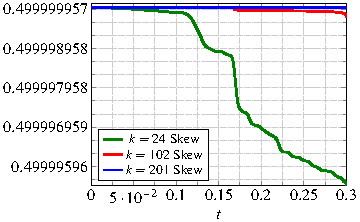
\includegraphics[scale=1]{Figures/paper-figure9.pdf}
%  \begin{tikzpicture}[scale=0.55]
%    \begin{axis}[xlabel=$t$,
%                 label style={font=\Large},
%                 legend pos=south west,
%                 legend entries={$k=24$ Skew,$k=102$ Skew,$k=201$ Skew},
%                 legend style={font=\large},
%                 grid=both,
%                 ticks=both,
%                 width=1.4\linewidth, 
%                 height=1.0\linewidth,
%                 minor x tick num=1,
%                 minor y tick num=2,	
%                 yticklabel style={/pgf/number format/.cd,fixed,precision=9},
%                 scaled x ticks = true,
%                 enlargelimits=false,
%                 scale only axis,
%                 ymax=0.5000001]
%                 \addplot[color=black!50!green,style=solid,style=ultra thick]  table[x = time, y = quantity] {./data/Compressible_Euler/1D/skew_symm_data/mass_24_1.txt};
%                 \addplot[color=red,style=solid,style=ultra thick]  table[x = time, y = quantity] {./data/Compressible_Euler/1D/skew_symm_data/mass_102_1.txt};
%                 \addplot[color=blue,style=solid,style=ultra thick]  table[x = time, y = quantity] {./data/Compressible_Euler/1D/skew_symm_data/mass_201_1.txt};
%    \end{axis}%  
%  \end{tikzpicture}
  \end{subfigure}
 % TOTAL MOMENTUM
  \begin{subfigure}[]{0.48\linewidth}
          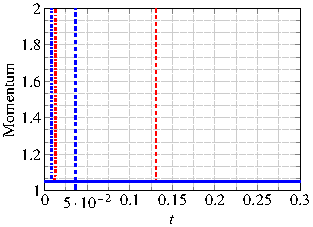
\includegraphics[scale=1]{Figures/paper-figure10.pdf}
%  \begin{tikzpicture}[scale=0.55]
%    \begin{axis}[ylabel = Momentum,
%                 xlabel=$t$,
%                 label style={font=\Large},
%                 legend pos=north east,
%                 %legend entries={$k=24$ Div,$k=102$ Div,$k=201$ Div,$k=24$ Skew,$k=102$ Skew,$k=201$ Skew},
%                 legend style={font=\large},
%                 grid=both,
%                 ticks=both,
%                 width=1.4\linewidth, 
%                 height=1.0\linewidth,
%                 minor x tick num=1,
%                 minor y tick num=2,	
%                 yticklabel style={/pgf/number format/.cd,fixed,precision=9},
%                 scaled x ticks = true,
%                 enlargelimits=false,
%                 scale only axis,
%                 ymin=1,
%                 ymax = 2,
%                 samples = 100]
%                 \addplot[color=red,style=dashdotted,style=ultra thick]  table[x = time, y = quantity] {./data/Compressible_Euler/1D/convective_data/momentum_102_1.txt};
%                 \addplot[color=blue,style=dashdotted,style=ultra thick]  table[x = time, y = quantity] {./data/Compressible_Euler/1D/convective_data/momentum_201_1.txt};
%                 \addplot[color=red,style=dashed,style=ultra thick]  table[x = time, y = quantity] {./data/Compressible_Euler/1D/divergence_data/momentum_102_1.txt};
%                 \addplot[color=blue,style=dashed,style=ultra thick]  table[x = time, y = quantity] {./data/Compressible_Euler/1D/divergence_data/momentum_201_1.txt};
%                 \addplot[color=red,style=solid,style=ultra thick]  table[x = time, y = quantity] {./data/Compressible_Euler/1D/skew_symm_data/momentum_102_1.txt};
%                 \addplot[color=blue,style=solid,style=ultra thick]  table[x = time, y = quantity] {./data/Compressible_Euler/1D/skew_symm_data/momentum_201_1.txt};
%    \end{axis}%  
%  \end{tikzpicture} 
  \end{subfigure}\hfill% 
 % TOTAL MOMENTUM (focus)
  \begin{subfigure}[]{0.48\linewidth}
          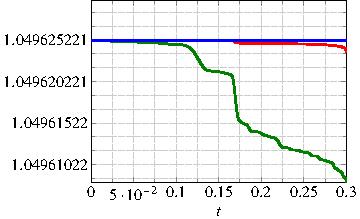
\includegraphics[scale=1]{Figures/paper-figure11.pdf}
%  \begin{tikzpicture}[scale=0.55]
%    \begin{axis}[xlabel=$t$,
%                 label style={font=\Large},
%                 legend pos=south west,
%                 legend style={font=\large},
%                 grid=both,
%                 ticks=both,
%                 width=1.4\linewidth, 
%                 height=1.0\linewidth,
%                 minor x tick num=1,
%                 minor y tick num=2,	
%                 yticklabel style={/pgf/number format/.cd,fixed,precision=9},
%                 scaled x ticks = true,
%                 enlargelimits=false,
%                 ymax=1.04963,
%                 scale only axis]
%                 \addplot[color=black!50!green,style=solid,style=ultra thick]  table[x = time, y = quantity] {./data/Compressible_Euler/1D/skew_symm_data/momentum_24_1.txt};
%                 \addplot[color=red,style=solid,style=ultra thick]  table[x = time, y = quantity] {./data/Compressible_Euler/1D/skew_symm_data/momentum_102_1.txt};
%                 \addplot[color=blue,style=solid,style=ultra thick]  table[x = time, y = quantity] {./data/Compressible_Euler/1D/skew_symm_data/momentum_201_1.txt};
%    \end{axis}%  
%  \end{tikzpicture}
  \end{subfigure}
 % ENERGY
  \begin{subfigure}[]{0.48\linewidth}
          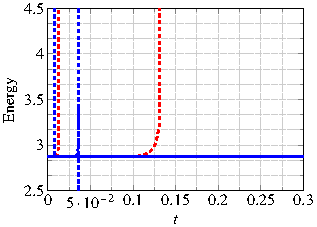
\includegraphics[scale=1]{Figures/paper-figure12.pdf}
%  \begin{tikzpicture}[scale=0.55]
%    \begin{axis}[ylabel = Energy,
%                 xlabel=$t$,
%                 label style={font=\Large},
%                 legend pos=north east,
%                 %legend entries={$k=24$ Div,$k=102$ Div,$k=201$ Div,$k=24$ Skew,$k=102$ Skew,$k=201$ Skew},
%                 legend style={font=\large},
%                 grid=both,
%                 ticks=both,
%                 width=1.4\linewidth, 
%                 height=1.0\linewidth,
%                 minor x tick num=1,
%                 minor y tick num=2,	
%                 yticklabel style={/pgf/number format/.cd,fixed,precision=9},
%                 scaled x ticks = true,
%                 enlargelimits=false,
%                 scale only axis,
%                 ymin=2.5,
%                 ymax = 4.5,
%                 samples = 100]
%                 \addplot[color=red,style=dashed,style=ultra thick]  table[x = time, y = quantity] {./data/Compressible_Euler/1D/convective_data/energy_102_1.txt};
%                 \addplot[color=blue,style=dashed,style=ultra thick]  table[x = time, y = quantity] {./data/Compressible_Euler/1D/convective_data/energy_201_1.txt};                
%                 \addplot[color=red,style=dashed,style=ultra thick]  table[x = time, y = quantity] {./data/Compressible_Euler/1D/divergence_data/energy_102_1.txt};
%                 \addplot[color=blue,style=dashed,style=ultra thick]  table[x = time, y = quantity] {./data/Compressible_Euler/1D/divergence_data/energy_201_1.txt};
%                 \addplot[color=red,style=solid,style=ultra thick]  table[x = time, y = quantity] {./data/Compressible_Euler/1D/skew_symm_data/energy_102_1.txt};
%                 \addplot[color=blue,style=solid,style=ultra thick]  table[x = time, y = quantity] {./data/Compressible_Euler/1D/skew_symm_data/energy_201_1.txt};
%    \end{axis}%  
%  \end{tikzpicture} 
  \caption{}
  \label{conservation_1D}
  \end{subfigure}\hfill% 
 % ENERGY (focus)
  \begin{subfigure}[]{0.48\linewidth}
          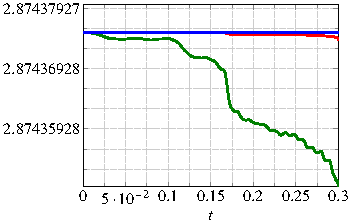
\includegraphics[scale=1]{Figures/paper-figure13.pdf}
%  \begin{tikzpicture}[scale=0.55]
%    \begin{axis}[xlabel=$t$,
%                 label style={font=\Large},
%                 legend pos=south west,
%                 legend style={font=\large},
%                 grid=both,
%                 ticks=both,
%                 width=1.4\linewidth, 
%                 height=1.0\linewidth,
%                 minor x tick num=1,
%                 minor y tick num=2,	
%                 yticklabel style={/pgf/number format/.cd,fixed,precision=9},
%                 scaled x ticks = true,
%                 enlargelimits=false,
%                 scale only axis,
%                 ymax = 2.87438]
%                 \addplot[color=black!50!green,style=solid,style=ultra thick]  table[x = time, y = quantity] {./data/Compressible_Euler/1D/skew_symm_data/energy_24_1.txt};
%                 \addplot[color=red,style=solid,style=ultra thick]  table[x = time, y = quantity] {./data/Compressible_Euler/1D/skew_symm_data/energy_102_1.txt};
%                 \addplot[color=blue,style=solid,style=ultra thick]  table[x = time, y = quantity] {./data/Compressible_Euler/1D/skew_symm_data/energy_201_1.txt};
%    \end{axis}%  
%  \end{tikzpicture}
  \caption{}
  \label{conservation_1D_focus}
  \end{subfigure}
  \caption{(\protect\subref{conservation_1D})  Evolution of the three conserved quantities for the reduced solution of the compressible Euler equation (mass, total momentum and total energy).  The divergent, advective and skew-symmetric formulations have been considered and $k=102,204$ basis are used in the reduced model. (\protect\subref{conservation_1D_focus}) Evolution of the conserved quantity for a stable reduced model using the skew-symmetric formulation.} 
  \label{fig:energy_pres_1D}
\end{figure}

%%%%%%%%%%%%%%%%%%%%%%%%%%%%%%%%%%%%%%%%%%%%
%%%%%%%%%%%%%%%% Approximation Error %%%%%%%%%%%%%%%%%
%%%%%%%%%%%%%%%%%%%%%%%%%%%%%%%%%%%%%%%%%%%%
\begin{figure}
\centering
\begin{subfigure}[]{0.48\linewidth}
        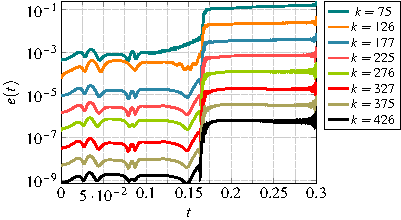
\includegraphics[scale=1]{Figures/paper-figure14.pdf}
%  \begin{tikzpicture}[scale=0.55]
%    \begin{semilogyaxis}[xlabel=$t$,
%                 ylabel=$e(t)$,
%                 label style={font=\Large},
%                 legend pos=outer north east,
%                 legend style={font=\large},
%                 legend entries={$k=75$,$k=126$,$k=177$,$k=225$,$k=276$,$k=327$,$k=375$,$k=426$},
%                 grid=both,
%                 ticks=both,
%                 width=1.4\linewidth, 
%                 height=1.0\linewidth,
%                 minor x tick num=1,
%                 minor y tick num=2,	
%                 yticklabel style={/pgf/number format/.cd,fixed,precision=9},
%                 scaled x ticks = true,
%                 enlargelimits=false,
%                 scale only axis,
%                 cycle list name=exotic]
%                 \addplot+[style=solid,style=ultra thick]  table[x = time, y = quantity] {./data/Compressible_Euler/1D/error/error_75.txt};  
%                 \addplot+[style=solid,style=ultra thick]  table[x = time, y = quantity] {./data/Compressible_Euler/1D/error/error_126.txt};      
%                 \addplot+[style=solid,style=ultra thick]  table[x = time, y = quantity] {./data/Compressible_Euler/1D/error/error_177.txt}; 
%                 \addplot+[style=solid,style=ultra thick]  table[x = time, y = quantity] {./data/Compressible_Euler/1D/error/error_225.txt};      
%                 \addplot+[style=solid,style=ultra thick]  table[x = time, y = quantity] {./data/Compressible_Euler/1D/error/error_276.txt};  
%                 \addplot+[style=solid,style=ultra thick]  table[x = time, y = quantity] {./data/Compressible_Euler/1D/error/error_327.txt}; 
%                 \addplot+[style=solid,style=ultra thick]  table[x = time, y = quantity] {./data/Compressible_Euler/1D/error/error_375.txt};      
%                 \addplot+[style=solid,style=ultra thick]  table[x = time, y = quantity] {./data/Compressible_Euler/1D/error/error_426.txt};              
%    \end{semilogyaxis}%  
%  \end{tikzpicture}
\end{subfigure}
\caption{Evolution in time of the error  between the high fidelity solution of the 1D compressible Euler and the reduced solution for different number of basis $k$. As error measure we consider $e(t)=\sqrt{\|\mathbf{r}-\mathbf{r}^r\|^2+\|\mathbf{ur}-\mathbf{ur}^r\|^2+\|\mathbf{p}-\mathbf{p}^r\|^2}$.}
\label{error_behaviour_1D}
\end{figure}

%%%%%%%%%%%%%%%%%%%%%%%%%%%%%%%%%%%%%%%%%%%%
%%%%%%%%%%%%% Snapshot of pressure and density %%%%%%%%%%%%%%
%%%%%%%%%%%%%%%%%%%%%%%%%%%%%%%%%%%%%%%%%%%%
\begin{figure}
\centering
\begin{subfigure}[t]{0.47\linewidth}
        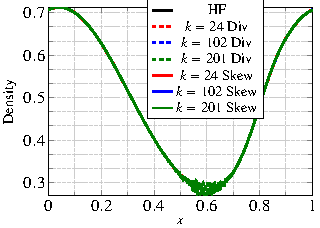
\includegraphics[scale=1]{Figures/paper-figure15.pdf}
%\begin{tikzpicture}[scale=0.58]
%    \begin{axis}[xlabel=$x$,
%                 ylabel=Density,
%                 label style={font=\large},
%                 %legend pos=south west,
%                 legend entries={HF,$k=24$ Div,$k=102$ Div,$k=201$ Div,$k=24$ Skew,$k=102$ Skew,$k=201$ Skew},
%                 legend style={font=\large},
%                 legend style={at={(axis cs:0.375,0.45)},anchor=south west},
%                 grid=both,
%                 ticks=both,
%                 width=1.4\linewidth, 
%                 height=1.0\linewidth,
%                 minor x tick num=1,
%                 minor y tick num=2,	
%                 yticklabel style={/pgf/number format/.cd,fixed,precision=9},
%                 scaled x ticks = true,
%                 enlargelimits=false,
%                 scale only axis]
%                 \addplot[color=black,style=solid,style=ultra thick]  table[x = time, y = energy] {./data/Compressible_Euler/1D/Snapshots/density_exact_300.txt};
%                 \addplot[color=red,style=dashed,style=ultra thick]  table[x = time, y = energy] {./data/Compressible_Euler/1D/Snapshots/density_approx_unstable_24_300.txt};
%                 \addplot[color=blue,style=dashed,style=ultra thick]  table[x = time, y = energy] {./data/Compressible_Euler/1D/Snapshots/density_approx_unstable_102_300.txt};
%                 \addplot[color=black!50!green,style=dashed,style=ultra thick]  table[x = time, y = energy] {./data/Compressible_Euler/1D/Snapshots/density_approx_unstable_201_300.txt};
%                 \addplot[color=red,style=solid,style=ultra thick]  table[x = time, y = energy] {./data/Compressible_Euler/1D/Snapshots/density_approx_24_300.txt};
%                 \addplot[color=blue,style=solid,style=ultra thick]  table[x = time, y = energy] {./data/Compressible_Euler/1D/Snapshots/density_approx_102_300.txt};
%                 \addplot[color=black!50!green,style=solid,style=ultra thick]  table[x = time, y = energy] {./data/Compressible_Euler/1D/Snapshots/density_approx_201_300.txt};
%    \end{axis}% 
%\end{tikzpicture}
\end{subfigure} 
\begin{subfigure}[t]{0.47\linewidth}
        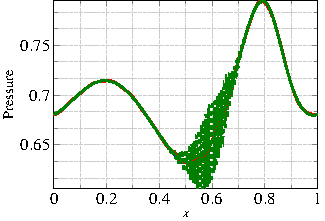
\includegraphics[scale=1]{Figures/paper-figure16.pdf}
%\begin{tikzpicture}[scale=0.58]
%    \begin{axis}[xlabel=$x$,
%                 ylabel=Pressure,
%                 label style={font=\large},
%                 legend pos=south west,
%                 %legend entries={HF,$k=24$ Div,$k=102$ Div,$k=201$ Div,$k=24$ Skew,$k=102$ Skew,$k=201$ Skew},
%                 legend style={font=\large},
%                 grid=both,
%                 ticks=both,
%                 width=1.4\linewidth, 
%                 height=1.0\linewidth,
%                 minor x tick num=1,
%                 minor y tick num=2,	
%                 yticklabel style={/pgf/number format/.cd,fixed,precision=9},
%                 scaled x ticks = true,
%                 enlargelimits=false,
%                 scale only axis]
%                 \addplot[color=black,style=solid,style=ultra thick]  table[x = time, y = energy] {./data/Compressible_Euler/1D/Snapshots/pressure_exact_300.txt};
%                 \addplot[color=red,style=dashed,style=ultra thick]  table[x = time, y = energy] {./data/Compressible_Euler/1D/Snapshots/pressure_approx_unstable_24_300.txt};
%                 \addplot[color=blue,style=dashed,style=ultra thick]  table[x = time, y = energy] {./data/Compressible_Euler/1D/Snapshots/pressure_approx_unstable_102_300.txt};
%                 \addplot[color=black!50!green,style=dashed,style=ultra thick]  table[x = time, y = energy] {./data/Compressible_Euler/1D/Snapshots/pressure_approx_unstable_201_300.txt};
%                 \addplot[color=red,style=solid,style=ultra thick]  table[x = time, y = energy] {./data/Compressible_Euler/1D/Snapshots/pressure_approx_24_300.txt};
%                 \addplot[color=blue,style=solid,style=ultra thick]  table[x = time, y = energy] {./data/Compressible_Euler/1D/Snapshots/pressure_approx_102_300.txt};
%                 \addplot[color=black!50!green,style=solid,style=ultra thick]  table[x = time, y = energy] {./data/Compressible_Euler/1D/Snapshots/pressure_approx_201_300.txt};
%    \end{axis}% 
%\end{tikzpicture}
\label{density_reduction}
\end{subfigure}

\begin{subfigure}[]{0.47\linewidth}
        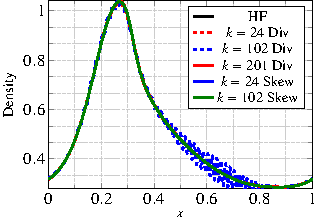
\includegraphics[scale=1]{Figures/paper-figure17.pdf}
%\begin{tikzpicture}[scale=0.58]
%    \begin{axis}[xlabel=$x$,
%                 ylabel=Density,
%                 label style={font=\large},
%                 legend pos=north east,
%                 legend entries={HF,$k=24$ Div,$k=102$ Div,$k=201$ Div,$k=24$ Skew,$k=102$ Skew,$k=201$ Skew},
%                 legend style={font=\large},
%                 grid=both,
%                 ticks=both,
%                 width=1.4\linewidth, 
%                 height=1.0\linewidth,
%                 minor x tick num=1,
%                 minor y tick num=2,	
%                 yticklabel style={/pgf/number format/.cd,fixed,precision=9},
%                 scaled x ticks = true,
%                 enlargelimits=false,
%                 scale only axis]
%                 \addplot[color=black,style=solid,style=ultra thick]  table[x = time, y = energy] {./data/Compressible_Euler/1D/Snapshots/density_exact_1000.txt};
%                 \addplot[color=red,style=dashed,style=ultra thick]  table[x = time, y = energy] {./data/Compressible_Euler/1D/Snapshots/density_approx_unstable_24_1000.txt};
%                 \addplot[color=blue,style=dashed,style=ultra thick]  table[x = time, y = energy] {./data/Compressible_Euler/1D/Snapshots/density_approx_unstable_102_1000.txt};
%                 \addplot[color=black!50!green,style=dashed,style=ultra thick]  table[x = time, y = energy] {./data/Compressible_Euler/1D/Snapshots/density_approx_unstable_201_1000.txt};
%                 \addplot[color=red,style=solid,style=ultra thick]  table[x = time, y = energy] {./data/Compressible_Euler/1D/Snapshots/density_approx_24_1000.txt};
%                 \addplot[color=blue,style=solid,style=ultra thick]  table[x = time, y = energy] {./data/Compressible_Euler/1D/Snapshots/density_approx_102_1000.txt};
%                 \addplot[color=black!50!green,style=solid,style=ultra thick]  table[x = time, y = energy] {./data/Compressible_Euler/1D/Snapshots/density_approx_201_1000.txt};
%    \end{axis}% 
%\end{tikzpicture}
\end{subfigure} 
\begin{subfigure}[]{0.47\linewidth}
        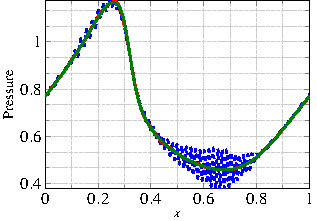
\includegraphics[scale=1]{Figures/paper-figure18.pdf}
%\begin{tikzpicture}[scale=0.58]
%    \begin{axis}[xlabel=$x$,
%                 ylabel=Pressure,
%                 label style={font=\large},
%                 legend pos=south west,
%                 %legend entries={HF,$k=24$ Div,$k=102$ Div,$k=201$ Div,$k=24$ Skew,$k=102$ Skew,$k=201$ Skew},
%                 legend style={font=\large},
%                 grid=both,
%                 ticks=both,
%                 width=1.4\linewidth, 
%                 height=1.0\linewidth,
%                 minor x tick num=1,
%                 minor y tick num=2,	
%                 yticklabel style={/pgf/number format/.cd,fixed,precision=9},
%                 scaled x ticks = true,
%                 enlargelimits=false,
%                 scale only axis]
%                 \addplot[color=black,style=solid,style=ultra thick]  table[x = time, y = energy] {./data/Compressible_Euler/1D/Snapshots/pressure_exact_1000.txt};
%                 \addplot[color=red,style=dashed,style=ultra thick]  table[x = time, y = energy] {./data/Compressible_Euler/1D/Snapshots/pressure_approx_unstable_24_1000.txt};
%                 \addplot[color=blue,style=dashed,style=ultra thick]  table[x = time, y = energy] {./data/Compressible_Euler/1D/Snapshots/pressure_approx_unstable_102_1000.txt};
%                 \addplot[color=black!50!green,style=dashed,style=ultra thick]  table[x = time, y = energy] {./data/Compressible_Euler/1D/Snapshots/pressure_approx_unstable_201_1000.txt};
%                 \addplot[color=red,style=solid,style=ultra thick]  table[x = time, y = energy] {./data/Compressible_Euler/1D/Snapshots/pressure_approx_24_1000.txt};
%                 \addplot[color=blue,style=solid,style=ultra thick]  table[x = time, y = energy] {./data/Compressible_Euler/1D/Snapshots/pressure_approx_102_1000.txt};
%                 \addplot[color=black!50!green,style=solid,style=ultra thick]  table[x = time, y = energy] {./data/Compressible_Euler/1D/Snapshots/pressure_approx_201_1000.txt};
%    \end{axis}% 
%\end{tikzpicture}
\end{subfigure}

\begin{subfigure}[]{0.47\linewidth}
        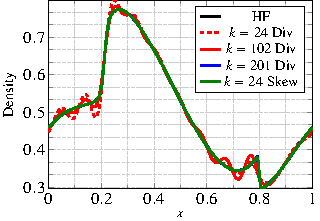
\includegraphics[scale=1]{Figures/paper-figure19.pdf}
%\begin{tikzpicture}[scale=0.58]
%    \begin{axis}[xlabel=$x$,
%                 ylabel=Density,
%                 label style={font=\large},
%                 legend pos=north east,
%                 legend entries={HF,$k=24$ Div,$k=102$ Div,$k=201$ Div,$k=24$ Skew,$k=102$ Skew,$k=201$ Skew},
%                 legend style={font=\large},
%                 grid=both,
%                 ticks=both,
%                 width=1.4\linewidth, 
%                 height=1.0\linewidth,
%                 minor x tick num=1,
%                 minor y tick num=2,	
%                 yticklabel style={/pgf/number format/.cd,fixed,precision=9},
%                 scaled x ticks = true,
%                 enlargelimits=false,
%                 scale only axis]
%                 \addplot[color=black,style=solid,style=ultra thick]  table[x = time, y = energy] {./data/Compressible_Euler/1D/Snapshots/density_exact_3000.txt};
%                 \addplot[color=red,style=dashed,style=ultra thick]  table[x = time, y = energy] {./data/Compressible_Euler/1D/Snapshots/density_approx_unstable_24_3000.txt};
%                 \addplot[color=blue,style=dashed,style=ultra thick]  table[x = time, y = energy] {./data/Compressible_Euler/1D/Snapshots/density_approx_unstable_102_3000.txt};
%                 \addplot[color=black!50!green,style=dashed,style=ultra thick]  table[x = time, y = energy] {./data/Compressible_Euler/1D/Snapshots/density_approx_unstable_201_3000.txt};
%                 \addplot[color=red,style=solid,style=ultra thick]  table[x = time, y = energy] {./data/Compressible_Euler/1D/Snapshots/density_approx_24_3000.txt};
%                 \addplot[color=blue,style=solid,style=ultra thick]  table[x = time, y = energy] {./data/Compressible_Euler/1D/Snapshots/density_approx_102_3000.txt};
%                 \addplot[color=black!50!green,style=solid,style=ultra thick]  table[x = time, y = energy] {./data/Compressible_Euler/1D/Snapshots/density_approx_201_3000.txt};
%    \end{axis}% 
%\end{tikzpicture}
\caption{}
\label{density_reduction_1D}
\end{subfigure} 
\begin{subfigure}[]{0.47\linewidth}
        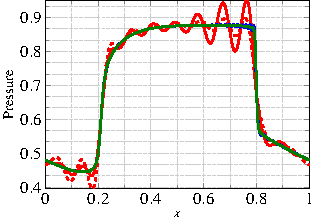
\includegraphics[scale=1]{Figures/paper-figure20.pdf}
%\begin{tikzpicture}[scale=0.58]
%    \begin{axis}[xlabel=$x$,
%                 ylabel=Pressure,
%                 label style={font=\large},
%                 legend pos=south west,
%                 %legend entries={HF,$k=24$ Div,$k=102$ Div,$k=201$ Div,$k=24$ Skew,$k=102$ Skew,$k=201$ Skew},
%                 legend style={font=\large},
%                 grid=both,
%                 ticks=both,
%                 width=1.4\linewidth, 
%                 height=1.0\linewidth,
%                 minor x tick num=1,
%                 minor y tick num=2,	
%                 yticklabel style={/pgf/number format/.cd,fixed,precision=9},
%                 scaled x ticks = true,
%                 enlargelimits=false,
%                 scale only axis]
%                 \addplot[color=black,style=solid,style=ultra thick]  table[x = time, y = energy] {./data/Compressible_Euler/1D/Snapshots/pressure_exact_3000.txt};
%                 \addplot[color=red,style=dashed,style=ultra thick]  table[x = time, y = energy] {./data/Compressible_Euler/1D/Snapshots/pressure_approx_unstable_24_3000.txt};
%                 \addplot[color=blue,style=dashed,style=ultra thick]  table[x = time, y = energy] {./data/Compressible_Euler/1D/Snapshots/pressure_approx_unstable_102_3000.txt};
%                 \addplot[color=black!50!green,style=dashed,style=ultra thick]  table[x = time, y = energy] {./data/Compressible_Euler/1D/Snapshots/pressure_approx_unstable_201_3000.txt};
%                 \addplot[color=red,style=solid,style=ultra thick]  table[x = time, y = energy] {./data/Compressible_Euler/1D/Snapshots/pressure_approx_24_3000.txt};
%                 \addplot[color=blue,style=solid,style=ultra thick]  table[x = time, y = energy] {./data/Compressible_Euler/1D/Snapshots/pressure_approx_102_3000.txt};
%                 \addplot[color=black!50!green,style=solid,style=ultra thick]  table[x = time, y = energy] {./data/Compressible_Euler/1D/Snapshots/pressure_approx_201_3000.txt};
%    \end{axis}% 
%\end{tikzpicture}
\caption{}
\label{pressure_reduction_1D}
\end{subfigure}
\caption{Qualitative comparison between different formulations for the reduced model in terms of density (\protect\subref{density_reduction_1D})  and pressure(\protect\subref{pressure_reduction_1D}) at $t=0.1,0.3$ and $1$s. Results for the advective formulation are not showed here because the related reduced solutions are unstable after a few time steps.}
\label{fig:snaps_1D_Euler}
\end{figure}

%%%%%%%%%%%%%%%%%%%%%%%%%%%%%%%%%%%%%%%%%
%%%%%%%%%%%%% Singular values 1D problem %%%%%%%%%%%%%%
%%%%%%%%%%%%%%%%%%%%%%%%%%%%%%%%%%%%%%%%%
\begin{figure}
\centering
        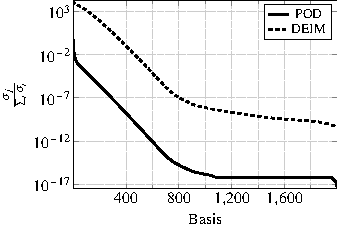
\includegraphics[scale=1]{Figures/paper-figure21.pdf}
%\begin{tikzpicture}[scale=0.5452]
%    \begin{semilogyaxis}[ylabel = $\frac{\sigma_j}{\sum_i \sigma_i}$,
%                 xlabel=Basis,
%                 label style={font=\Large},
%                 legend style={font=\large},
%                 legend entries = {POD,DEIM},
%                 grid=both,
%                 ticks=both,
%                 width=0.7\linewidth, 
%                 height=0.5\linewidth,
%                 minor x tick num=1,
%                 minor y tick num=2,	
%                 yticklabel style={/pgf/number format/.cd,fixed,precision=9},
%                 scaled x ticks = true,
%                 enlargelimits=false,
%                 scale only axis,
%                 samples = 100,
%                 xtick = {400, 800, 1200, 1600}]
%                 \addplot[color=black,style=solid,style=ultra thick]  table[x = n, y = sing_values] {./data/Compressible_Euler/1D/Singular_values/sv.txt};
%                 \addplot[color=black,style=dashed,style=ultra thick]  table[x = n, y = sv] {./data/Compressible_Euler/1D/Singular_values/sv_DEIM.txt};
%    \end{semilogyaxis}
%\end{tikzpicture}
\caption{Decay of the singular values of the snapshot matrix related to POD and DEIM algorithms for the 1D compressible Euler problem.}
\label{fig:singular_values_decay_1D}
\end{figure}

\begin{figure}[h!]
\centering
\begin{subfigure}[]{0.47\linewidth}
        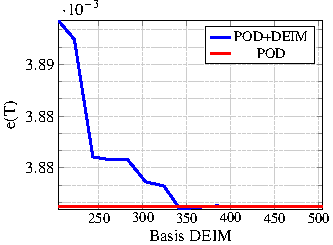
\includegraphics[scale=1]{Figures/paper-figure22.pdf}
%\begin{tikzpicture}[scale=0.58]
%    \begin{axis}[ylabel = e(T),
%                 xlabel=Basis DEIM,
%                 label style={font=\Large},
%                 legend pos=north east,
%                 legend entries={POD+DEIM,POD},
%                 legend style={font=\large},
%                 grid=both,
%                 ticks=both,
%                 width=1.4\linewidth, 
%                 height=1\linewidth,
%%                 minor x tick num=1,
%                 minor y tick num=2,	
%                 xticklabel style={font = \large},
%%                 yticklabel style={/pgf/number format/.cd,fixed,precision=9},
%                 scaled x ticks = true,
%                 enlargelimits=false,
%                 scale only axis]
%                 \addplot[color=blue,style=solid,style=ultra thick]  table[x = time, y = quantity] {./data/Compressible_Euler/1D/error_DEIM/error_DEIM.txt};      
%                 \addplot[color=red,style=solid,style=ultra thick]  table[x = time, y = quantity] {./data/Compressible_Euler/1D/error_DEIM/error_POD.txt};
%    \end{axis}
%\end{tikzpicture}
\caption{}
\label{error_DEIM}
\end{subfigure}
\begin{subfigure}[]{0.47\linewidth}
        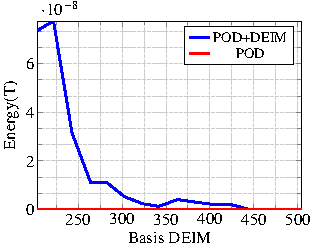
\includegraphics[scale=1]{Figures/paper-figure23.pdf}
%\begin{tikzpicture}[scale=0.58]
%    \begin{axis}[ylabel = Energy(T),
%                 xlabel=Basis DEIM,
%                 label style={font=\Large},
%                 legend pos=north east,
%                 legend entries={POD+DEIM,POD},
%                 legend style={font=\large},
%                 grid=both,
%                 ticks=both,
%                 width=1.4\linewidth, 
%                 height=1\linewidth,
%                 minor x tick num=1,
%                 minor y tick num=2,	
%%                 yticklabel style={/pgf/number format/.cd,fixed,precision=9},
%                 scaled x ticks = true,
%                 enlargelimits=false,
%                 scale only axis]
%                 \addplot[color=blue,style=solid,style=ultra thick]  table[x = time, y = quantity] {./data/Compressible_Euler/1D/error_DEIM/error_energy_DEIM.txt};      
%                 \addplot[color=red,style=solid,style=ultra thick]  table[x = time, y = quantity] {./data/Compressible_Euler/1D/error_DEIM/error_energy_POD.txt};
%    \end{axis}
%\end{tikzpicture}
\caption{}
\label{energy_DEIM}
\end{subfigure}
\caption{Comparison between standard POD and POD with DEIM treatment of the nonlinear term in terms of the error (\protect\subref{error_DEIM}) and the total energy (\protect\subref{energy_DEIM}).}
\label{fig:RIC2}
\end{figure}


